%%%%%%%%%%%%%%%%%%%%%%%%%%%%%%%%%%%%%%
% Multiplicative domain poster
% Created by Nathaniel Johnston
% August 2009
% http://www.nathanieljohnston.com/index.php/2009/08/latex-poster-template/
%%%%%%%%%%%%%%%%%%%%%%%%%%%%%%%%%%%%%%

\documentclass[final]{beamer}
\usepackage[scale=1.24]{beamerposter}
\usepackage{graphicx}			% allows us to import images
\usepackage{listings}

%-----------------------------------------------------------
% Custom commands that I use frequently
%-----------------------------------------------------------

\newcommand{\bb}[1]{\mathbb{#1}}
\newcommand{\cl}[1]{\mathcal{#1}}
\newcommand{\fA}{\mathfrak{A}}
\newcommand{\fB}{\mathfrak{B}}
\newcommand{\Tr}{{\rm Tr}}
\newtheorem{thm}{Theorem}

%-----------------------------------------------------------
% Define the column width and poster size
% To set effective sepwid, onecolwid and twocolwid values, first choose how many columns you want and how much separation you want between columns
% The separation I chose is 0.024 and I want 4 columns
% Then set onecolwid to be (1-(4+1)*0.024)/4 = 0.22
% Set twocolwid to be 2*onecolwid + sepwid = 0.464
%-----------------------------------------------------------

\newlength{\sepwid}
\newlength{\onecolwid}
\newlength{\twocolwid}
\setlength{\paperwidth}{44in}
\setlength{\paperheight}{34in}
\setlength{\sepwid}{0.024\paperwidth}
\setlength{\onecolwid}{0.22\paperwidth}
\setlength{\twocolwid}{0.464\paperwidth}
\setlength{\topmargin}{-0.5in}
\usetheme{confposter}
\usepackage{exscale}
\usebackgroundtemplate {
\includegraphics[width=\paperwidth,height=\paperheight,
keepaspectratio]{poster-background.pdf}}

%-----------------------------------------------------------
% Define colours (see beamerthemeconfposter.sty to change these colour definitions)
%-----------------------------------------------------------

\setbeamercolor{block title}{fg=norange}
\setbeamercolor{block body}{fg=black}
\setbeamercolor{block alerted title}{fg=white,bg=dblue!70}
\setbeamercolor{block alerted body}{fg=black,bg=dblue!10}



\pagecolor{bg=dblue!10}

%-----------------------------------------------------------
% Name and authors of poster/paper/research
%-----------------------------------------------------------

\title{Alternative High Performance Benchmarks}
\author{Kurt R. Rudolph}
\institute{Department of Computer Science, University of Illinois Urbana-Champaign}

%-----------------------------------------------------------
% Start the poster itself
%-----------------------------------------------------------
% The \rmfamily command is used frequently throughout the poster to force a serif font to be used for the body text
% Serif font is better for small text, sans-serif font is better for headers (for readability reasons)
%-----------------------------------------------------------

\begin{document}
\begin{frame}[t]
	\begin{columns}[t]												% the [t] option aligns the column's content at the top
		\begin{column}{\sepwid}\end{column}			% empty spacer column
			\begin{column}{\onecolwid}
				\begin{block}{Unified Parallel C (UPC)}
					A partitioned global address space (PGAS) language that extends C. Specifically, UPC employs \emph{shared pointers} which enabling the threads of a program access to a common address space.
					\lstinputlisting[language=C, basicstyle=\footnotesize]{ upcSample.c}
					The UPC example above distributes the work of computing a dot product across all available threads in the program. 
				\end{block}
				\vspace{2 mm}
				\begin{alertblock}{UPC Issues}
					\begin{itemize}
						\item Internal consistency issues.
						\item Blocking index computation.
							\begin{itemize}
							\item Great load balancing 
							\item Computability issues
							\end{itemize}
						\item Mixing with MPI 2-sided communication generally leads to chaos.
							\begin{itemize}
								\item Compiler needs to know about any current communicators to correctly calculate an index.
							\end{itemize}
						\item Pointer arithmetic is rather costly.
					\end{itemize}
				\end{alertblock}
					The results to the right were taken on the NCSA Blue-Print cluster.  The cluster employs 64 nodes, each node supporting 16 power5 processing cores and 64GB of memory.  Both the MPI and UPC timing results were taken utilizing 1 to 64 nodes with 16 processes per node accordingly.  \\
					\tiny{\rmfamily{\begin{thebibliography}{99}
					\bibitem{MPI2} MPI-2: Extensions to the Message-Passing Interface, Message Passing Interface Forum, July 18, 1997.
					\bibitem{ElG03a} Tarek A. El-Ghazawi, William W. Carlson, Jesse M. Draper. UPC Language Specifications V1.1 (http://upc.gwu.edu). March, 2003.
					 \bibitem{Car99} William W. Carlson, Jesse M. Draper. Introduction to UPC and language specification CCS-TR-99-157.
					 \end{thebibliography}}}
			\end{column}
			\begin{column}{\sepwid}\end{column}			% empty spacer column
			\begin{column}{\twocolwid}
				\begin{alertblock}{Abstract}
					\rmfamily{
						Benchmarks for High-Performance clusters generally focus on floating-point intensive calculations. Few of these address data intensive graph operations, a class of computation increasingly growing in demand.  As an alternative to standard floating-point benchmarks such as LinPack, a new benchmark, the Graph 500, has been proposed. The benchmark employ's multiple implementations with the intention to identify desecrate performance aspects via the comparative results, however a PGAS model has yet to be developed. This project focuses on early understanding of the capabilities a Graph 500 UPC implementation offers. Specifically: 1. the UPC expressibility for irregular graph operations of Graph500 2. simple performance testing the efficiency of UPC with runs up to 1024 cores.
					}
				\end{alertblock}
				\begin{block}{The Graph 500 Benchmark}
					A data intensive benchmark comparing graph operations and implemented in a variety of parallel programming models, the Graph 500 provides insight into performance aspects of HPC systems not normally seen in most floating-point benchmarks. 
					
					The benchmark is composed of two kernels. The first kernel is a scalable data generator component which produces the edge tuples of the graph.  The second kernel is the graph traversal component.  Within the second kernel, 64 random search keys are selected from the node of the generated  graph and a breadth-first search is performed for each key. Both kernels are timed and verified.
					
					The UPC implementation of this project offers the additional perspective of a partitioned global address space model and further identify discrepancies in HPC system performance.
				\end{block}
				\begin{block}{Timing Results}
					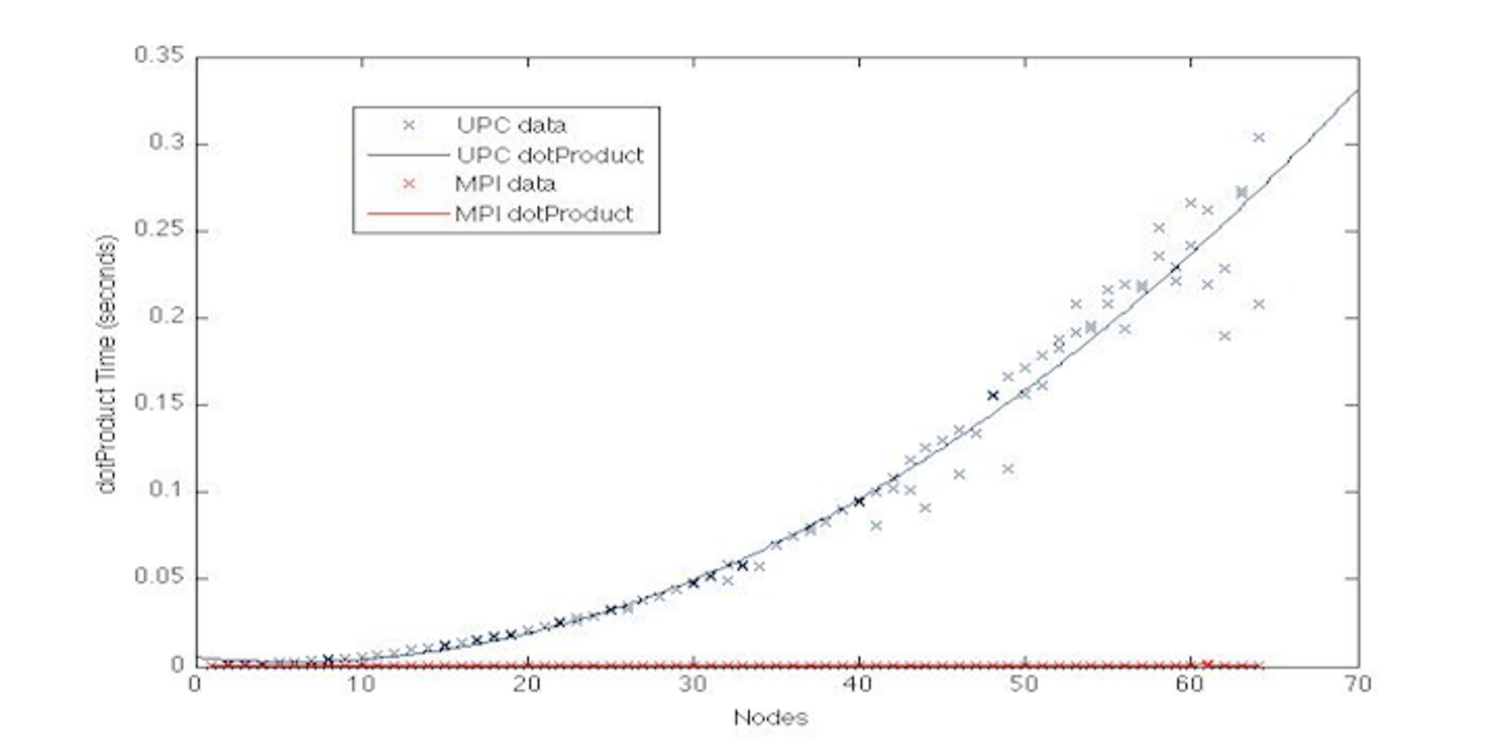
\includegraphics[width=\twocolwid, keepaspectratio]{DotProduct.pdf}\\
				\end{block}						
			\end{column}	
			\begin{column}{\sepwid}\end{column}			% empty spacer column
			\begin{column}{\onecolwid}
				\begin{block}{The Graph500 BFS}
					The Graph 500 employs multiple implementations using MPI and OpenMP.  
					
					The "Simple" MPI implementation achieves two-sided communication through communicator functions such as  \emph{send} and \emph{receive}. Sample from Graph500 BFS MPI Simple:\vspace{2 mm}
					\lstinputlisting[language=C, basicstyle=\footnotesize]{ mpiSimpleSample.c}
					 \vspace{5 mm}
					  The "One Sided" MPI implementation achieves one-sided communication through MPI \emph{windows}, a feature built into MPICH2 API.  When a thread creates an MPI \emph{window} access to another threads address space is enabled through the variables associated through that window.  Sample from the Graph500 BFS MPI One Sided: 
					  \vspace{2 mm}
					  \lstinputlisting[language=C, basicstyle=\footnotesize]{ mpiOneSidedSample.c} 
					  \vspace{5 mm}
					  The UPC implementation of this project does not require "windows" to achieve one sided communication.  However, address space used in any collective operations needs to be allocated in shared memory space and receives the according performance loss of accessing a shared pointer over a local pointer.  Sample from the projects' Graph500 BFS UPC implementation: 
					  \vspace{2 mm}
					  \lstinputlisting[language=C, basicstyle=\footnotesize]{ upcOneSidedSample.c} 
				\end{block}
		\end{column}
		\begin{column}{\sepwid}\end{column}			% empty spacer column
	 \end{columns}
\end{frame}
\end{document}

































